% tex file for results

% from regression_results

\noindent \textbf{Pre-Processing}

Smoothing performed well in reducing outliers and extreme values in the time-series per voxel. We used a value of $\sigma=1$ for the Gaussian smoothing.  We performed HRF convolution and time correction as well with success.
\vspace{5mm}

\noindent \textbf{Model Selection}

For our linear regression model, we ended up choosing the deisgn matrix model with a single HRF feature with all conditions, a linear drift feature, and three pairs of Fourier features. The dimension of our final feature matrix is time $\times$ 9. 
\vspace{5mm}

\noindent \textbf{Normality Test}

Based on the Shapiro-Wilk test for normality on the residuals with a p-value threshold of 0.05, we found that the normality assumptions of the linear models were violated roughly 35\% of the time. This suggests that we should be cautious of the validity of hypothesis testing and possibly explore alternatives for analyzing the coefficients.
\vspace{5mm}

\noindent \textbf{Clustering}

Our end goal was to identify regions of the brain that are associated with the neurological stimulus by way of the hemodynamic response. In pursuing this goal, we utilized the $\hat{\beta}$ and t-statistics corresponding to the HRF coefficient of the chosen linear model design matrix. Based on the fact that the normality assumptions did not hold for a large proportion of the voxels, we utilized analyses that both relied and did not rely on the normality assumption.

We used two perspectives to cluster, one based of multiple correction and another based on hierarchical clustering using Ward's method. Hierarchical clustering was computationally costly against the large number of voxels and was not feasible. We used 3 different approaches to multiple comparison correction. 
\vspace{5mm}

\noindent \textbf{Multiple Comparison}

The most canonical appraoch we used was Benjamini Hochberg (BH), which utilized p-statistics. This type of analysis assumes normality of the $\hat{\beta}$ values, which we saw where not always the case. BH also required unique threshold values for each person, which was a large draw-back. We additionally utilized a quantile-based clustering of the t-stat values and $\hat{\beta}$ values. These provided more interpretable clusters across subjects and produced similar results indicating consistency.
\vspace{5mm}

\noindent \textbf{Identifying Active Regions}

We considered the results from each of the approaches for clustering with multiple comparison corrections. As alluded to previously, the BH approach was less interpretable and required per-subject tuning of parameters to obtain logical results. So, it was generally a less favorable approach than the t-statistic and $\hat{\beta}$ quantile-based clustering. 

Sub 1, Kent's actual, 
[Some plots here for at least 2 subjects with consistent results and at least 1 subject with weird results. Ideally should also compare methods to demonstrate the similarities between t and beta and the weirdness of BH.]

A region consistently identified with high HRF activity across subjects for the t-statistic and $\hat{\beta}$ approaches was the front area of the brain. Other areas with potentially high activity include a small region toward the center and back and some areas on the left edge. 
\vspace{5mm}


\begin{figure}[ht]
\centering
\begin{minipage}[b]{0.45\linewidth}
	\centering
	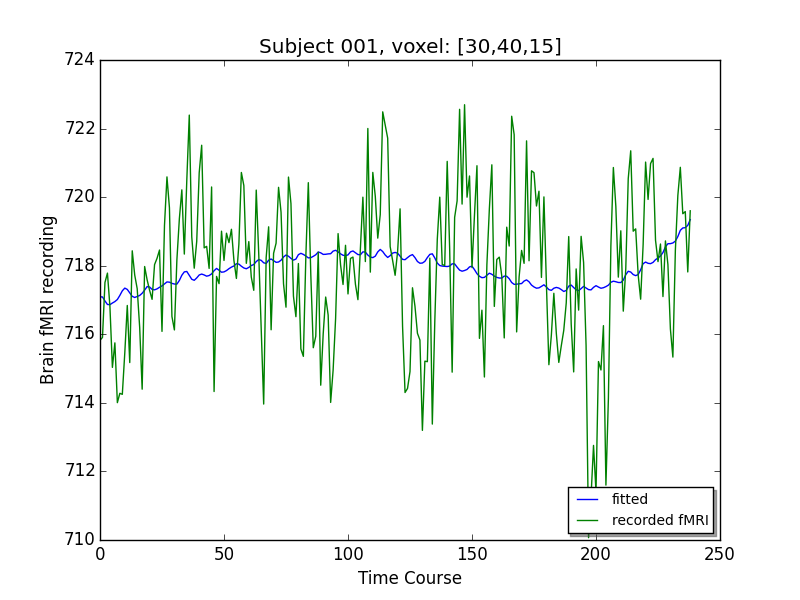
\includegraphics[width=.8\linewidth]{../images/Fitted_v_Actual.png} 
	\caption{Fitted/Predicted vs Actual fMRI BOLD contrast}
	\label{fig:fit_vs_act}
\end{minipage}	
\quad
\begin{minipage}[b]{0.45\linewidth}
	\centering
		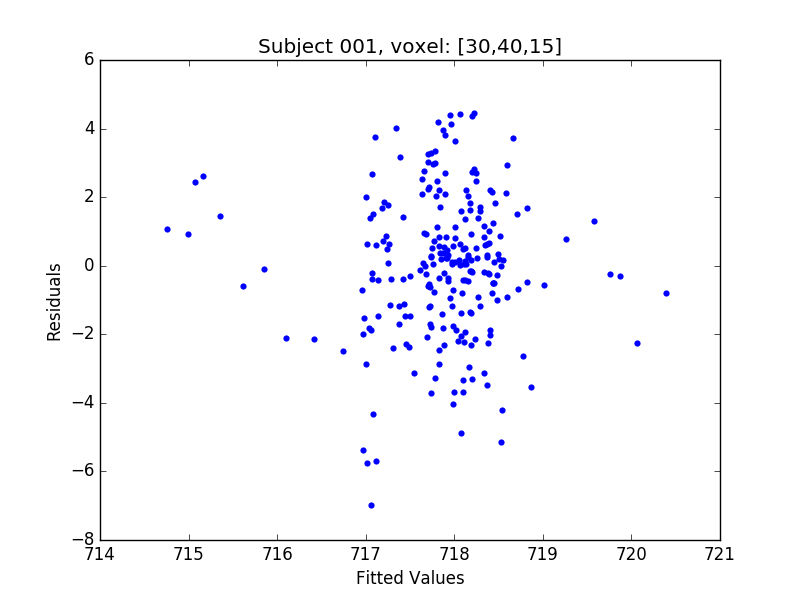
\includegraphics[width=.8\linewidth]{../images/Fitted_v_Residuals.png} 
	\caption{Fitted fMRI BOLD contrast vs Residual from Linear Regression}
	\label{fig:fit_vs_res}
\end{minipage}
\end{figure}





  
\begin{figure}[ht]
\centering
\begin{minipage}[b]{0.45\linewidth}
	\centering
	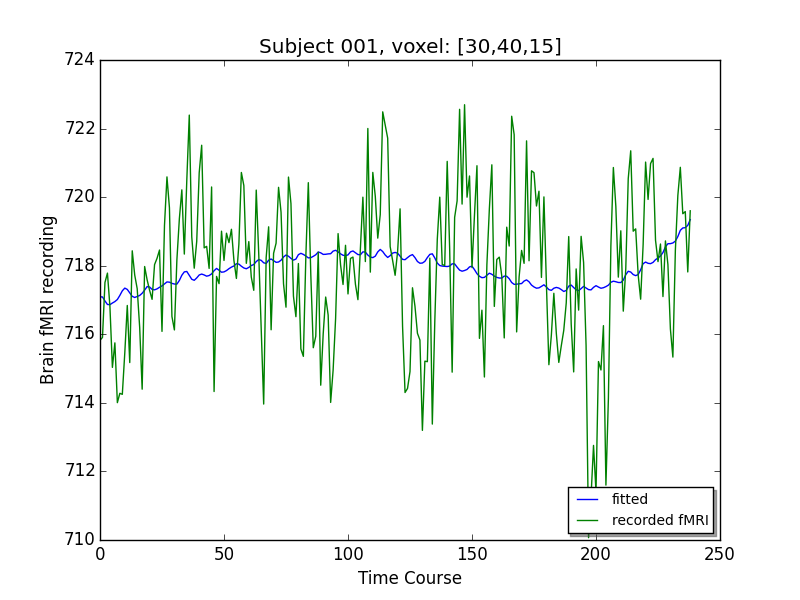
\includegraphics[width=.8\linewidth]{../images/Fitted_v_Actual.png} 
	\caption{Fitted/Predicted vs Actual fMRI BOLD contrast}
	\label{fig:fit_vs_act}
\end{minipage}	
\quad
\begin{minipage}[b]{0.45\linewidth}
	\centering
		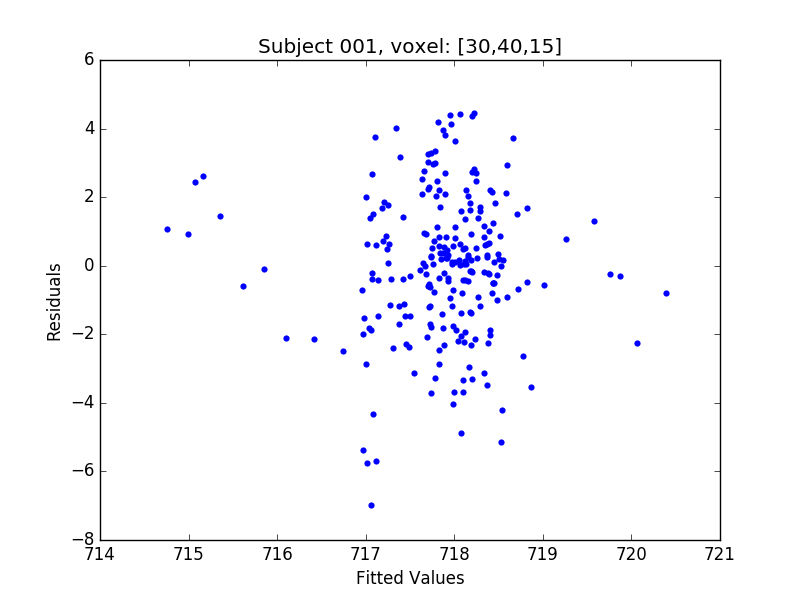
\includegraphics[width=.8\linewidth]{../images/Fitted_v_Residuals.png} 
	\caption{Fitted fMRI BOLD contrast vs Residual from Linear Regression}
	\label{fig:fit_vs_res}
\end{minipage}
\end{figure}




%\begin{figure}[ht]
%\centering
%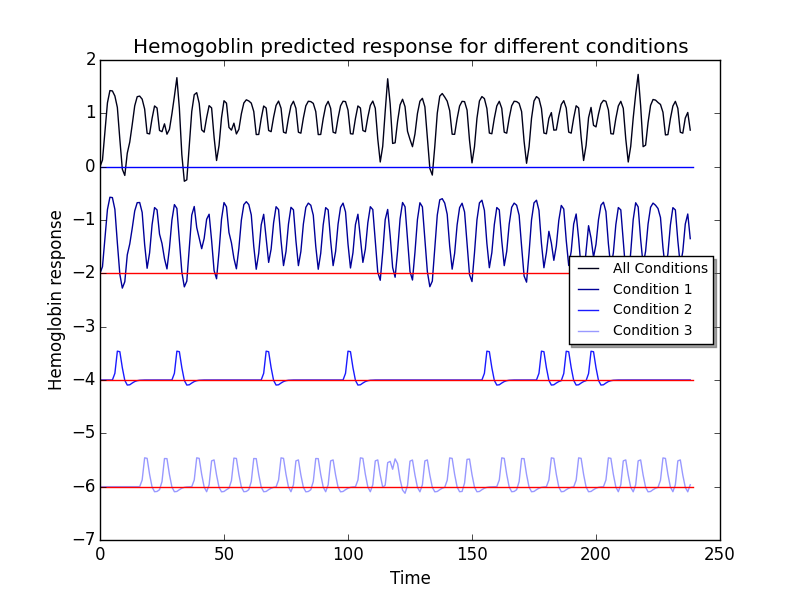
\includegraphics[scale=.5]{../images/all_cond_time}  
%\caption{Plotting all predicted HR for conditions.}
%\label{fig:all_cond_time}
%\end{figure}

*****As we also obtained $\hat{\beta}$ values (coefficients) from the linear 
regression models, we looked at the 3-dimensional reports of the 
$\hat{\beta}$ values, a less rigorous analysis than hypothesis testing with 
t-statistics [Figure reference]. $\sim$Remove or update****



The numerous other multiple regression models discussed in 
\textit{Linear Regression} should be analyzed similarly in the future. 



% from hypothesis_results
% tex file for hypothesis testing results 
\par \indent The results of our simple linear regression t-statistic 
comparisons across subjects are shown in [Figure \ref{fig:ht}]. We can see 
each slice of the brain from top to bottom in each section of the image. The 
blue areas shows parts of the brain that had a negative t-statistic while the 
red parts of the image shows parts of the brain that had a positive t-
statistic.

\begin{figure}[ht] \centering
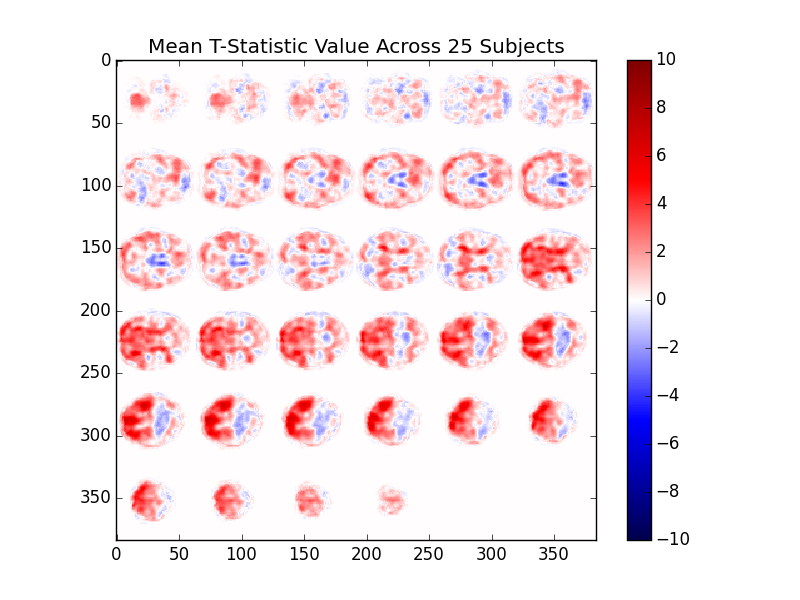
\includegraphics[scale=0.5]{../images/hypothesis_testing} \caption{Across-subject 
mean of t-Statistic per voxel.} \label{fig:ht} \end{figure}

\par The parts of the image that were cut out by the mask are white so we can 
more clearly see the contrast in our results. Based on a cursory look at this 
image, we can see a pattern of dark red (high positive t-statistics) in the lower 
left parts of the brain, and area of dark blue (high negative t-statistics) in 
the center and lower middle parts parts of the brain.


